% arXiv-style preprint: the basic building blocks under the Kasami "Almost Bent" proof.
% Build with a Unicode engine (arXiv supports both):
%   tectonic  kasami-ab-foundations.tex
%   xelatex   kasami-ab-foundations.tex   (run twice for references)
% The Lean snippets keep their real unicode, rendered with a unicode mono font.
\documentclass[11pt]{article}

\usepackage[margin=1.25in]{geometry}
\usepackage{amsmath,amssymb}
\usepackage{xcolor}
\usepackage{fontspec}
\usepackage{listings}
\usepackage{tikz}
\usepackage{tikz-cd}
\usepackage{pgfplots}
\pgfplotsset{compat=1.16}
\usetikzlibrary{positioning,arrows.meta,fit,backgrounds}

\usepackage{parskip}          % whitespace between paragraphs
\setlength{\parskip}{1.0em}
\linespread{1.13}

% A unicode monospace font so Lean glyphs (ℕ, →, ≠, ∀, ∑, ...) render directly.
\newfontfamily\leanmono{DejaVu Sans Mono}[Scale=0.85]

% --- a light Lean style for listings -----------------------------------------
\definecolor{leanbg}{gray}{0.97}
\definecolor{leankw}{rgb}{0.30,0.20,0.65}
\definecolor{leancm}{rgb}{0.35,0.45,0.35}
\lstdefinestyle{lean}{
  backgroundcolor=\color{leanbg},
  basicstyle=\leanmono\small,
  keywordstyle=\color{leankw}\bfseries,
  commentstyle=\color{leancm}\itshape,
  morekeywords={def,theorem,lemma,structure,where,fun,Prop,Finset,Type,
    univ,filter,card,instance,variable,namespace,end,open,noncomputable,
    if,then,else,Field,Fintype,CharP,Odd,Nat,import},
  morecomment=[l]{--},
  columns=fullflexible,
  keepspaces=true,
  showstringspaces=false,
  frame=single,
  framesep=6pt,
  xleftmargin=4pt,
  aboveskip=1.1em, belowskip=1.1em,
  extendedchars=true,
}
\lstset{style=lean}
% ------------------------------------------------------------------------------

\title{\bf The Foundations under ``Kasami is Almost Bent''\\[3pt]
  \large A Picture Book of the Basic Building Blocks}
\author{}
\date{}

\begin{document}
\maketitle

\begin{abstract}\noindent
This note shows the \emph{lowest} pieces that hold up a Lean~4 proof:
the Kasami power map $x \mapsto x^{d}$ is \emph{Almost Bent}.

The proof stands on \textbf{two pillars} that meet at the top.
Each pillar stands on its own \textbf{leaf} that touches Mathlib directly.
We draw the shape first, then walk up it.

Every block gets a small picture and the matching Lean snippet.
The English is kept plain on purpose.
\end{abstract}

\bigskip

% =====================================================================
\section{The shape of the proof}

The whole proof is a small tree.

At the bottom are three \textbf{leaves}.
A leaf is a file that imports \emph{only} Mathlib.
So a leaf sits straight on top of Mathlib, with nothing in between.

The three leaves are
\[
  \textsf{AutBase} \qquad \textsf{Lemma31} \qquad \textsf{APN/Defs} .
\]

Above the leaves are \textbf{two pillars}.

\begin{center}
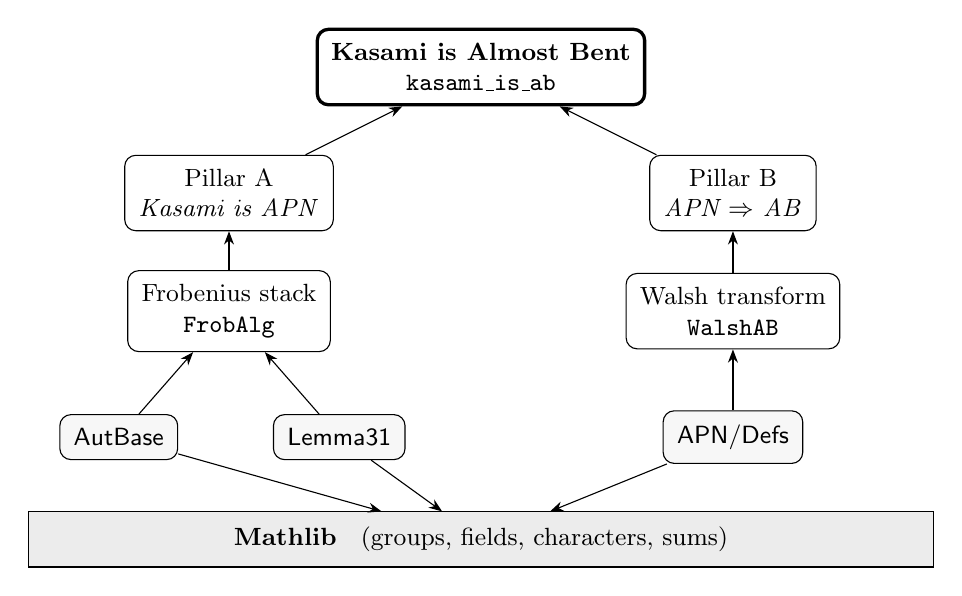
\begin{tikzpicture}[
  every node/.style={font=\small},
  box/.style={draw,rounded corners,align=center,inner sep=5pt,fill=white},
  leaf/.style={draw,rounded corners,align=center,inner sep=5pt,fill=leanbg},
  >=Stealth
]
  % top
  \node[box,very thick] (top) at (0,4.2) {\textbf{Kasami is Almost Bent}\\ \texttt{kasami\_is\_ab}};

  % pillars
  \node[box] (apn)  at (-3.2,2.6) {Pillar A\\ \emph{Kasami is APN}};
  \node[box] (ab)   at ( 3.2,2.6) {Pillar B\\ \emph{APN $\Rightarrow$ AB}};

  % middle helpers
  \node[box] (frob) at (-3.2,1.1) {Frobenius stack\\ \texttt{FrobAlg}};
  \node[box] (walsh)at ( 3.2,1.1) {Walsh transform\\ \texttt{WalshAB}};

  % leaves
  \node[leaf] (autb) at (-4.6,-0.5) {\textsf{AutBase}};
  \node[leaf] (lem)  at (-1.8,-0.5) {\textsf{Lemma31}};
  \node[leaf] (defs) at ( 3.2,-0.5) {\textsf{APN/Defs}};

  % mathlib bar
  \node[draw,fill=gray!15,minimum width=11.5cm,minimum height=0.7cm] (ml) at (0,-1.8) {\textbf{Mathlib} \; (groups, fields, characters, sums)};

  \draw[->] (apn) -- (top);
  \draw[->] (ab)  -- (top);
  \draw[->] (frob) -- (apn);
  \draw[->] (walsh) -- (ab);
  \draw[->] (autb) -- (frob);
  \draw[->] (lem)  -- (frob);
  \draw[->] (defs) -- (walsh);
  \draw[->] (autb) -- (ml);
  \draw[->] (lem)  -- (ml);
  \draw[->] (defs) -- (ml);
\end{tikzpicture}
\end{center}

Read the picture bottom to top.

\textbf{AutBase} feeds only the left pillar (Kasami is APN), through the
Frobenius stack.

\textbf{APN/Defs} feeds the right pillar (APN $\Rightarrow$ AB), through the
Walsh transform.  This path \emph{skips} AutBase.

So the top theorem reaches Mathlib in two ways at once:
partly through AutBase, partly on its own.
That is the one fact to keep in mind.

% =====================================================================
\section{Leaf 1 --- AutBase: a twisted multiply}

The first leaf studies one very simple map.
Pick a constant $a$.  Raise the input to a power of the characteristic,
then multiply by $a$:
\[
  T_r(a)\colon\quad x \;\longmapsto\; a \cdot x^{\,p^{r}} .
\]

Because $x \mapsto x^{p}$ is the Frobenius map, $T_r(a)$ is ``Frobenius, then
scale''.  These maps are the alphabet of the whole APN pillar.

\begin{center}
\begin{tikzcd}[column sep=large,row sep=large]
  x \arrow[r,"x^{p^r}"] \arrow[rr,bend right=28,"T_r(a)"'] & x^{p^r} \arrow[r,"\cdot\,a"] & a\,x^{p^r}
\end{tikzcd}
\end{center}

\begin{lstlisting}
-- RequestProject/FiniteField/AutBase.lean   (imports only Mathlib)
def semilinearOp (r : ℕ) (a : F) (x : F) : F := a * x ^ (p ^ r)
\end{lstlisting}

We also track \emph{which} powers actually show up in an additive polynomial.
That set of indices is the \emph{support}.

\begin{lstlisting}
noncomputable def support (n : ℕ) (coeffs : Fin n → F) : Finset (Fin n) :=
  Finset.univ.filter fun i => coeffs i ≠ 0
\end{lstlisting}

% =====================================================================
\section{Leaf 2 --- Lemma31: turn a product into a difference}

The second leaf is one clean trick.

Take a linear map $L$ and a multiplicative map $M$.
Look at the product map
\[
  P(x) \;=\; L(x)\cdot M(x) .
\]

The trick: \emph{$P$ is injective exactly when a family of difference maps are
all bijective.}  This swaps a hard product question for an easy linear one.

\begin{center}
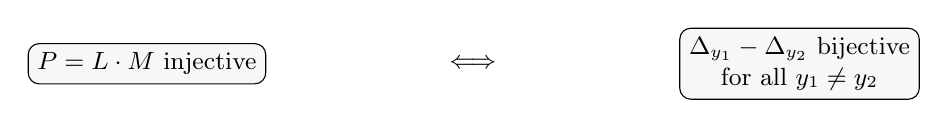
\begin{tikzpicture}[every node/.style={font=\small},>=Stealth,node distance=10mm]
  \node[draw,rounded corners,fill=leanbg] (p) {$P=L\cdot M$ injective};
  \node[right=22mm of p] (mid) {$\Longleftrightarrow$};
  \node[draw,rounded corners,fill=leanbg,align=center,right=22mm of mid] (d)
    {$\Delta_{y_1}-\Delta_{y_2}$ bijective\\ for all $y_1\neq y_2$};
\end{tikzpicture}
\end{center}

\begin{lstlisting}
-- RequestProject/FiniteField/Lemma31.lean   (imports only Mathlib)
def PMap31 (L : F →ₗ[K] F) (M : F → F) (x : F) : F := L x * M x

lemma PMap31_inj_iff_Delta_sub_bij (L : F →ₗ[K] F) {M : F → F}
    (hM : ∀ a b, M (a * b) = M a * M b) (hMinj : Function.Injective M) :
    Function.Injective (PMap31 L M) ↔
    ∀ y₁ y₂ : F, y₁ ≠ y₂ → Function.Bijective (Delta L M y₁ - Delta L M y₂)
\end{lstlisting}

% =====================================================================
\section{Leaf 3 --- APN/Defs: the Kasami exponent}

The third leaf just \emph{names} the objects of the right pillar.

The star is the \textbf{Kasami exponent}
\[
  d(k) \;=\; 2^{2k} - 2^{k} + 1 .
\]

The helper is the \textbf{linearized polynomial}
\[
  L_k(x) \;=\; x^{2^{k}} + x ,
\]
which is additive: $L_k(x+y) = L_k(x) + L_k(y)$.

\begin{center}
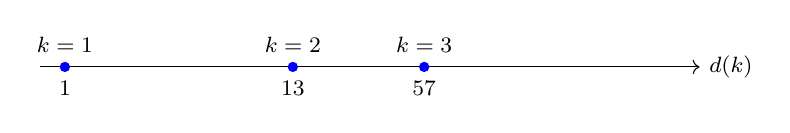
\begin{tikzpicture}[scale=0.62,every node/.style={font=\footnotesize}]
  % a tiny "exponent" number line marking d for small k
  \draw[->] (-0.5,0)--(13,0) node[right]{$d(k)$};
  \foreach \k/\v in {1/1,2/13,3/57} {
     \pgfmathsetmacro\x{ln(\v)/ln(3)*2.0 }
     \fill[blue] (\x,0) circle (3pt);
     \node[above] at (\x,0.1) {$k=\k$};
     \node[below] at (\x,-0.1) {$\v$};
  }
\end{tikzpicture}

{\small The first Kasami exponents: $d(1)=1,\; d(2)=13,\; d(3)=57$.}
\end{center}

\begin{lstlisting}
-- RequestProject/APN/Defs.lean   (imports only Mathlib)
def d (k : ℕ) : ℕ := 2 ^ (2 * k) - 2 ^ k + 1

def L (k : ℕ) (x : F) : F := x ^ (2 ^ k) + x
\end{lstlisting}

% =====================================================================
\section{The glue --- Frobenius arithmetic}

Both pillars lean on one fact about finite fields.

A nonzero element $x$ satisfies $x^{|F|-1}=1$.
So an exponent only matters \emph{modulo} $|F|-1$:
\[
  a \equiv b \pmod{|F|-1} \;\Longrightarrow\; x^{a} = x^{b} .
\]

This is the wrap-around that lets us slide exponents freely.

\begin{center}
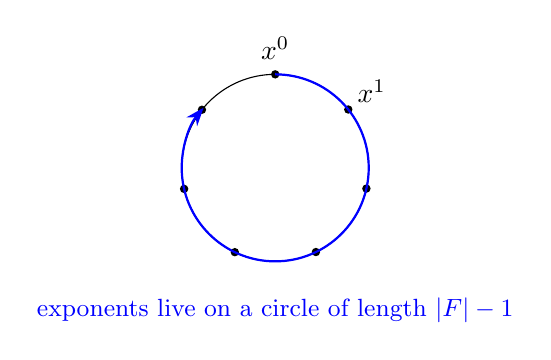
\begin{tikzpicture}[scale=0.95,>=Stealth]
  \def\R{1.25}
  \draw (0,0) circle (\R);
  \foreach \i in {0,...,6}{
     \fill (90-\i*51.4:\R) circle (1.6pt);
  }
  \node at (90:\R+0.35) {$x^0$};
  \node at (90-51.4:\R+0.4) {$x^1$};
  \draw[->,blue,thick] (90:\R) arc (90:-220:\R);
  \node[blue] at (0,-1.9) {\small exponents live on a circle of length $|F|-1$};
\end{tikzpicture}
\end{center}

\begin{lstlisting}
-- RequestProject/FiniteField/FrobAlg.lean  (the Dempwolff--Müller stack)
lemma pow_eq_pow_of_mod_eq {x : F} (hx : x ≠ 0) {a b : ℕ}
    (hab : a % (Fintype.card F - 1) = b % (Fintype.card F - 1)) :
    x ^ a = x ^ b
\end{lstlisting}

% =====================================================================
\section{Pillar A --- Kasami is APN}

\textbf{APN} means: in every nonzero direction $a$, the difference equation
\[
  (x+a)^{d} + x^{d} = b
\]
has at most two solutions.

The proof of this pillar uses AutBase (the twisted multiplies) and the
Frobenius glue.  It shows two distinct inputs cannot collide.

\begin{center}
\begin{tikzpicture}[scale=0.8,every node/.style={font=\small}]
  \draw[->] (-0.2,0)--(5,0) node[right]{$x$};
  \draw[->] (0,-0.2)--(0,3.2) node[above]{$x^{d}$};
  % a few graph dots; mark the only allowed double-hit
  \foreach \x/\y in {0.5/0.5, 1.3/1.9, 2.1/0.9, 2.9/2.6, 3.7/1.4, 4.4/0.4}
    \fill[blue] (\x,\y) circle (2pt);
  \draw[<->,red] (1.3,1.9)--(2.1,0.9);
  \node[red] at (2.6,1.7) {at most a pair};
\end{tikzpicture}

{\small APN: no nonzero direction sends three inputs to the same value.}
\end{center}

\begin{lstlisting}
-- RequestProject/Kasami/Classical/KasamiAPN.lean
theorem kasami_is_apn {F : Type*} [Field F] [Fintype F] [CharP F 2]
    {n : ℕ} (hn : Fintype.card F = 2 ^ n) (k : ℕ)
    (hk : 1 < k) (hk_odd : Odd k) (hkn : k < n)
    (hn_odd : Odd n) (hcop : Nat.Coprime k n) :
    IsAPN (fun (x : F) => x ^ (kasamiExp k))
\end{lstlisting}

% =====================================================================
\section{Pillar B --- the Walsh transform and AB}

The right pillar measures the map with \textbf{characters}.

Let $\chi(x) = +1$ if the trace of $x$ is $0$, else $-1$.
The \textbf{Walsh coefficient} sums this sign over all inputs:
\[
  W(a,b) \;=\; \sum_{x} \chi\bigl(a\,x + b\,f(x)\bigr).
\]

A map is \textbf{Almost Bent (AB)} when every squared Walsh value is flat ---
only two bars are allowed:
\[
  W(a,b)^2 \in \{\,0,\; 2^{\,n+1}\,\} \qquad (a \neq 0).
\]

\begin{center}
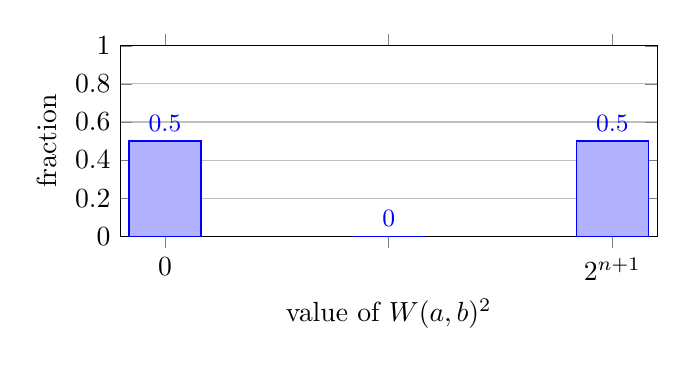
\begin{tikzpicture}
\begin{axis}[
   ybar, width=8.4cm, height=4.0cm,
   ymin=0, ymax=1, xtick={0,1,2},
   xticklabels={$0$,,$2^{n+1}$},
   xlabel={value of $W(a,b)^2$}, ylabel={fraction},
   bar width=26pt, ymajorgrids,
   nodes near coords, every node near coord/.append style={font=\small},
]
\addplot coordinates {(0,0.5) (1,0) (2,0.5)};
\end{axis}
\end{tikzpicture}

{\small An AB map: the Walsh spectrum has only two heights.}
\end{center}

\begin{lstlisting}
-- RequestProject/Walsh/WalshAB.lean   (rooted in Mathlib via APN/Defs)
noncomputable def walsh (f : F → F) (a b : F) : ℤ :=
  ∑ x : F, χ (a * x + b * f x)

noncomputable def IsAB {n : ℕ} (_ : Fintype.card F = 2 ^ n) (f : F → F) : Prop :=
  ∀ a : F, a ≠ 0 → ∀ b : F,
    walsh f a b ^ 2 = 0 ∨ walsh f a b ^ 2 = (2 ^ (n + 1) : ℤ)
\end{lstlisting}

The pillar itself is the step \emph{APN $\Rightarrow$ AB} for $n$ odd.
It works because the fourth moment of the Walsh values is pinned by the APN
count, and each squared value is divisible by $2^{n+1}$, so it can only be
$0$ or $2^{n+1}$.

\begin{lstlisting}
-- RequestProject/Kasami/Classical/KasamiABProof.lean
theorem apn_power_implies_ab
    {n : ℕ} (hn : Fintype.card F = 2 ^ n) (hn_odd : Odd n) (hn_pos : 1 < n)
    (d : ℕ) (hd : Nat.Coprime d (2 ^ n - 1)) (hd_pos : 0 < d)
    (h_apn : KasamiAPN.IsAPN (fun x : F => x ^ d)) :
    IsAlmostBent hn (fun x : F => x ^ d)
\end{lstlisting}

% =====================================================================
\section{The top --- the two pillars meet}

Now join the pillars.

Pillar A gives ``Kasami is APN''.
Pillar B turns any APN power map into an AB map.
Put them together and the crown follows.

\begin{center}
\begin{tikzcd}[column sep=2.4cm,row sep=large]
  \textsf{AutBase}\;,\ \textsf{Lemma31} \arrow[d] &
  \textsf{APN/Defs} \arrow[d] \\
  \boxed{\text{Kasami is APN}} \arrow[dr] &
  \boxed{\text{APN}\Rightarrow\text{AB}} \arrow[d] \\
  & \boxed{\textbf{Kasami is AB}}
\end{tikzcd}
\end{center}

\begin{lstlisting}
-- RequestProject/Kasami/Classical/KasamiABProof.lean
theorem kasami_is_ab_proven
    {n : ℕ} (hn : Fintype.card F = 2 ^ n) (k : ℕ)
    (hk : 1 < k) (hkn : k < n)
    (hn_odd : Odd n) (hcop : Nat.Coprime k n) :
    IsAlmostBent hn (fun (x : F) => x ^ (kasamiExp k)) :=
  apn_power_implies_ab hn hn_odd (by linarith) (kasamiExp k)
    (kasami_exp_coprime_general hk hkn hcop hn_odd)
    (by unfold kasamiExp; omega)
    (kasami_is_apn_general hn k hk hkn hn_odd hcop)
\end{lstlisting}

% =====================================================================
\section{One sentence to remember}

\textsf{AutBase} is a real Mathlib-rooted leaf --- but it is \emph{not} the
single base.

There are three leaves.
\textsf{AutBase} (with \textsf{Lemma31}) holds up the APN pillar.
\textsf{APN/Defs} holds up the AB pillar, skipping \textsf{AutBase}.

So the top AB theorem rests on Mathlib \emph{partly through AutBase, and partly
on its own}.

\bigskip
\begin{center}\small
Three leaves, two pillars, one crown.
\end{center}

\end{document}
